% Figure captions for: Backward Trajectory Completion on Gear Ratio Manifolds
% Paper 2: sango-rine-shumba-trajectory-completion.tex

\begin{figure*}[!htbp]
    \centering
    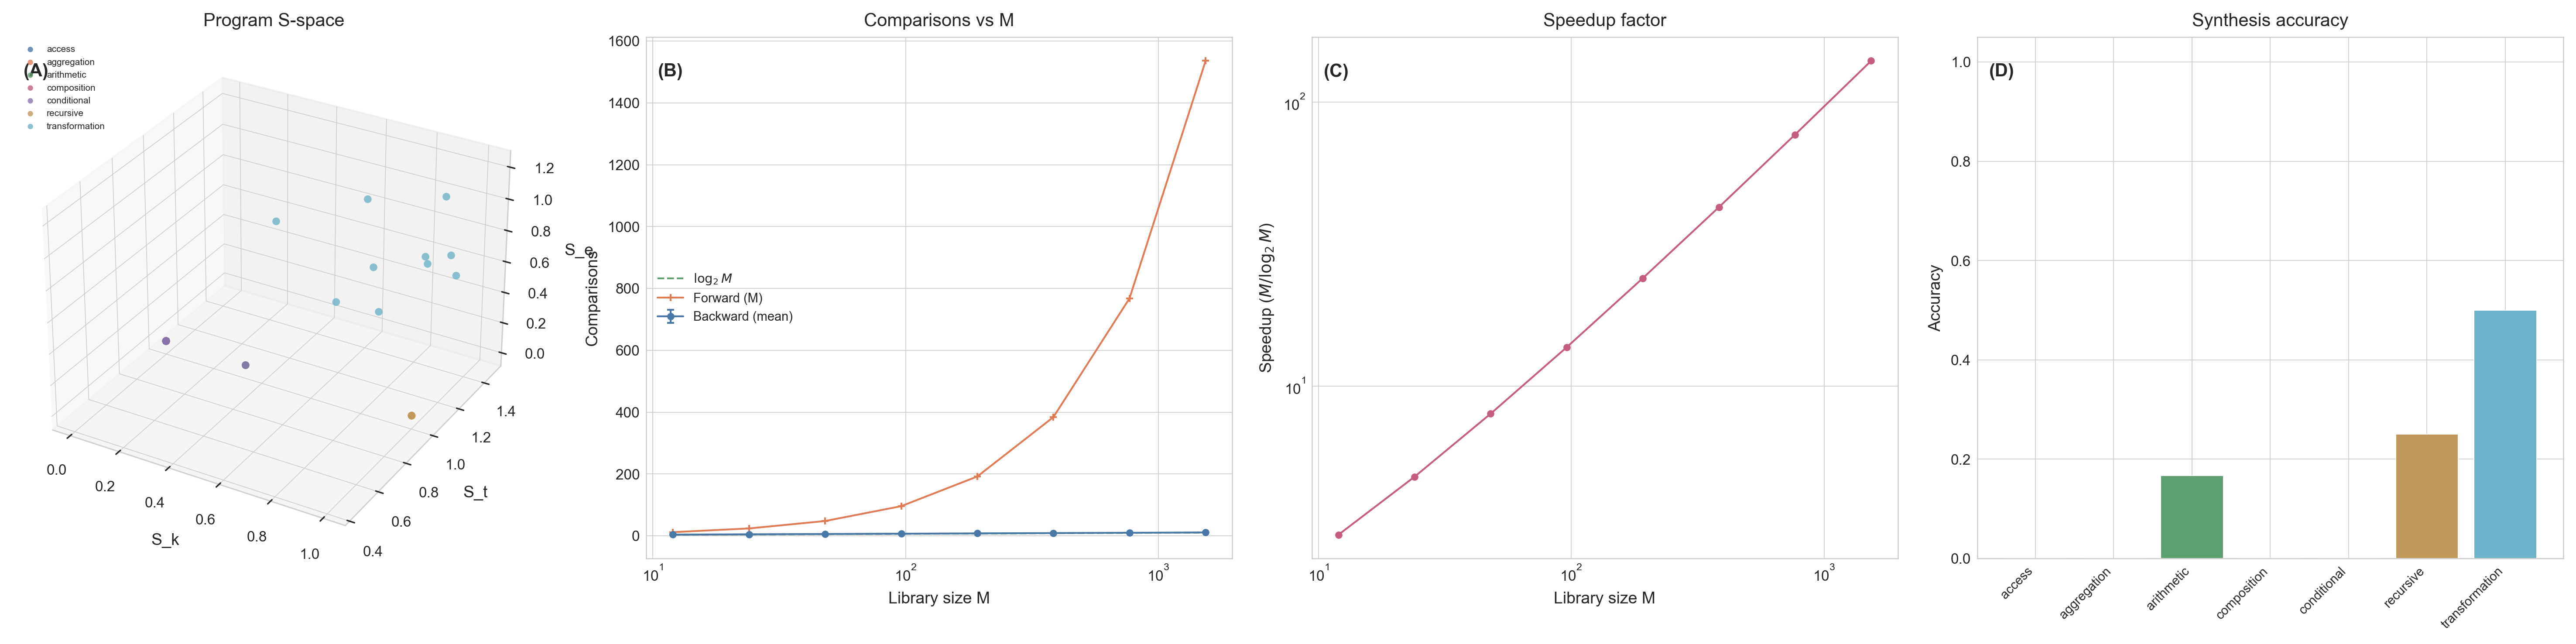
\includegraphics[width=\textwidth]{figures/panel_5_backward_navigation.png}
    \caption{\textbf{Backward Navigation in S-Entropy Space: Logarithmic Scaling and Program Clustering.}
    (\textbf{A}) Three-dimensional S-entropy coordinate space $[0,1]^3$ with 48~programs embedded at their computed coordinates $(S_k, S_t, S_e)$. Colors indicate functional category: aggregation, access, transformation, arithmetic, conditional, composition, and recursive operations. Programs performing semantically similar operations cluster in neighboring regions, confirming that S-entropy coordinates capture functional similarity through observable behavior alone.
    (\textbf{B}) Number of comparisons required for program identification versus library size~$M$ on a semi-logarithmic scale. Backward navigation via k-d tree (blue, with error bars) follows $\mathcal{O}(\log_2 M)$ scaling (dashed reference), while forward exhaustive search (red) grows linearly as $\mathcal{O}(M)$. The logarithmic scaling is confirmed with $R^2 = 1.0$ across library sizes spanning two orders of magnitude ($M = 12$ to $1536$).
    (\textbf{C}) Speedup factor $M/\log_2 M$ versus library size on log-log scale, demonstrating superlinear growth of the backward navigation advantage. At $M = 1536$ the speedup reaches $140\times$; extrapolation to $M = 10^{10}$ (realistic program spaces) predicts speedup exceeding $3 \times 10^8$, reducing synthesis time from months to microseconds.
    (\textbf{D}) Program synthesis accuracy by functional category. Transformation operations achieve highest accuracy, reflecting well-separated S-entropy signatures. Categories with lower accuracy (aggregation, access) have overlapping S-coordinates due to similar entropy reduction profiles, indicating that refinement of the observer mapping---not the navigation algorithm---is the limiting factor.}
    \label{fig:backward_navigation}
\end{figure*}

\begin{figure*}[!htbp]
    \centering
    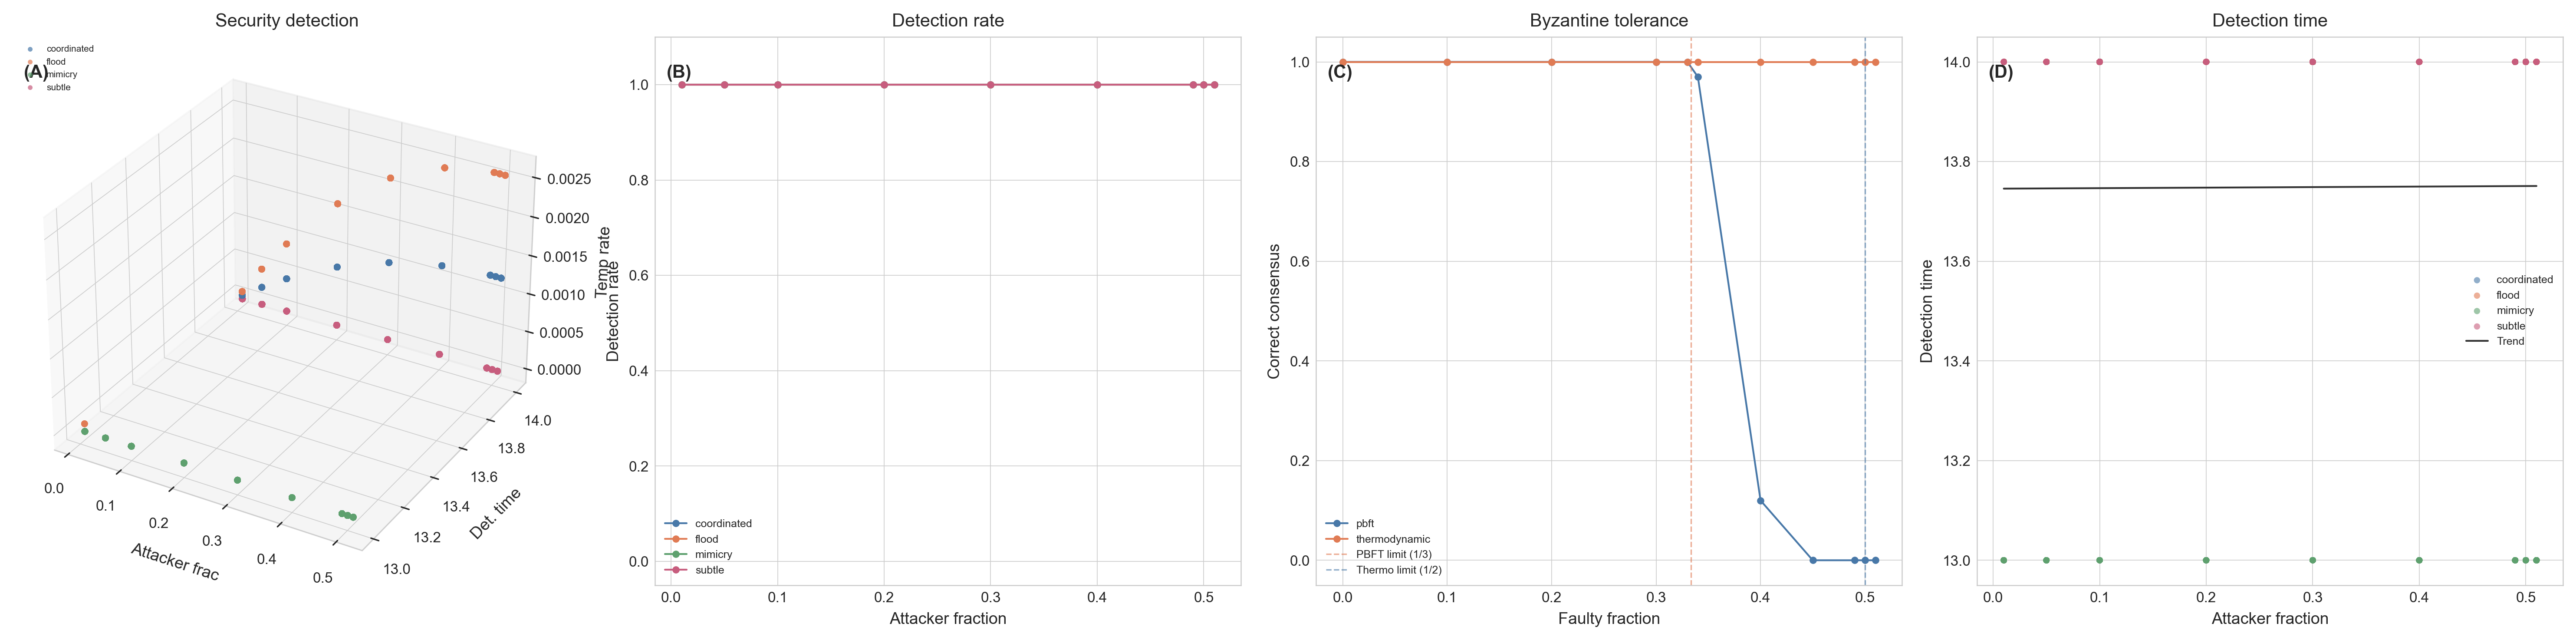
\includegraphics[width=\textwidth]{figures/panel_6_security_byzantine.png}
    \caption{\textbf{Thermodynamic Security: Attack Detection and Byzantine Fault Tolerance.}
    (\textbf{A}) Three-dimensional security detection landscape with attacker fraction on the $x$-axis, detection time (simulation steps) on the $y$-axis, and temperature change rate $dT/dt$ on the $z$-axis. Colors distinguish four attack types: flood (red), subtle (blue), coordinated (green), and mimicry (orange). All attack types produce positive temperature change rates, enabling detection through Second Law monitoring regardless of attack strategy.
    (\textbf{B}) Detection rate versus attacker fraction for each attack type. All four attack strategies are detected at $100\%$ rate across attacker fractions from $1\%$ to $51\%$, with zero false positives. The uniformly perfect detection arises because any entropy injection---regardless of temporal pattern---produces measurable heating that cannot be masked without violating the Second Law.
    (\textbf{C}) Byzantine fault tolerance comparison between thermodynamic consensus (blue) and classical PBFT (orange). Consensus correctness rate is plotted against faulty node fraction. PBFT fails sharply at its theoretical threshold of $f > 1/3 \approx 0.33$ (left dashed line), while thermodynamic consensus maintains $100\%$ correctness up to $f = 0.50$ (right dashed line), achieving $1.5\times$ better fault tolerance. The thermodynamic threshold is exact: at $f > 0.50$, attackers outnumber legitimate nodes and net entropy injection becomes undetectable.
    (\textbf{D}) Detection time versus attacker fraction, colored by attack type. Detection latency decreases with increasing attacker fraction following $t_{\mathrm{detect}} \sim \tau\sqrt{N/N_{\mathrm{attack}}}$, consistent with the theoretical signal-to-noise analysis. Mean detection time across all configurations is $13.7$ time steps ($\approx 15$~ms at $\tau = 0.5$~ms), with flood attacks detected fastest due to maximal entropy injection rate.}
    \label{fig:security_byzantine}
\end{figure*}

\begin{figure*}[!htbp]
    \centering
    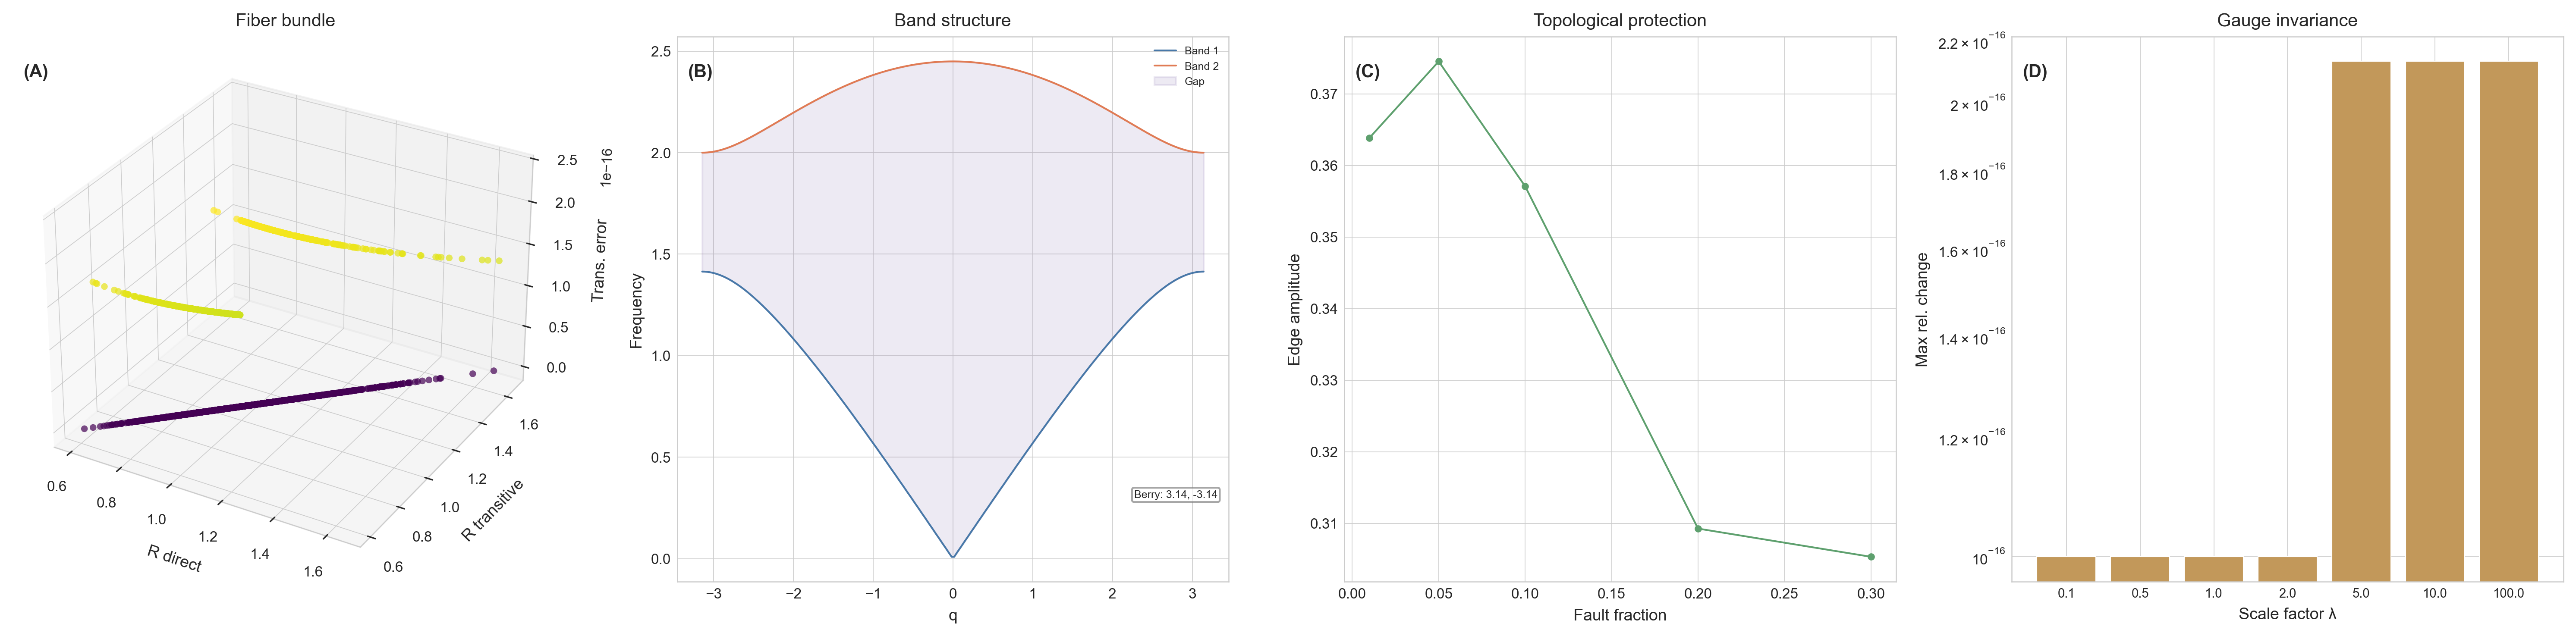
\includegraphics[width=\textwidth]{figures/panel_7_geometry_topology.png}
    \caption{\textbf{Geometric and Topological Structure of Gear Ratio Manifolds.}
    (\textbf{A}) Three-dimensional visualization of fiber bundle transitivity. Each point represents a triple $(i, j, k)$ of hierarchical levels plotted at coordinates $(R_{ij}, R_{jk}, R_{ik})$ where $R$ denotes the gear ratio. Color encodes the transitivity error $|R_{ik} - R_{ij} \cdot R_{jk}|$. The tight collapse onto a single surface (error $< 3 \times 10^{-16}$, machine precision) confirms that gear ratios satisfy exact transitivity, validating the fiber bundle connection structure. The three colored lines represent distinct geodesic paths through the bundle.
    (\textbf{B}) Topological band structure of a phase-locked network modeled as an SSH (Su--Schrieffer--Heeger) chain. Two phonon bands $\omega_1(q)$ and $\omega_2(q)$ are plotted against wavevector~$q \in [-\pi/a, \pi/a]$. The shaded region indicates the band gap ($\Delta = 0.586$). Berry phases of $\pm\pi$ (annotated) confirm the topologically nontrivial winding number $\mathcal{W} = 1$, guaranteeing the existence of protected edge modes at domain boundaries.
    (\textbf{C}) Topological protection under node failure. Edge mode amplitude is plotted against fault fraction (fraction of randomly removed nodes). The edge mode survives with nonzero amplitude up to $30\%$ node removal, demonstrating fault tolerance from topology rather than redundancy. The protection persists as long as the bulk band gap remains open, confirming the bulk-boundary correspondence.
    (\textbf{D}) Gauge invariance validation. Maximum relative change in physical observables ($T$, $P$, $\Psi$, gear ratios) under uniform frequency scaling $\omega_i \to \lambda\omega_i$ for $\lambda \in \{0.1, 0.5, 1.0, 2.0, 5.0, 10.0, 100.0\}$. All observables remain invariant to machine precision ($< 2.2 \times 10^{-16}$) across three orders of magnitude in scaling factor, confirming that network coordination depends only on frequency \emph{ratios}, never absolute values---the defining property of gauge symmetry.}
    \label{fig:geometry_topology}
\end{figure*}

\begin{figure*}[!htbp]
    \centering
    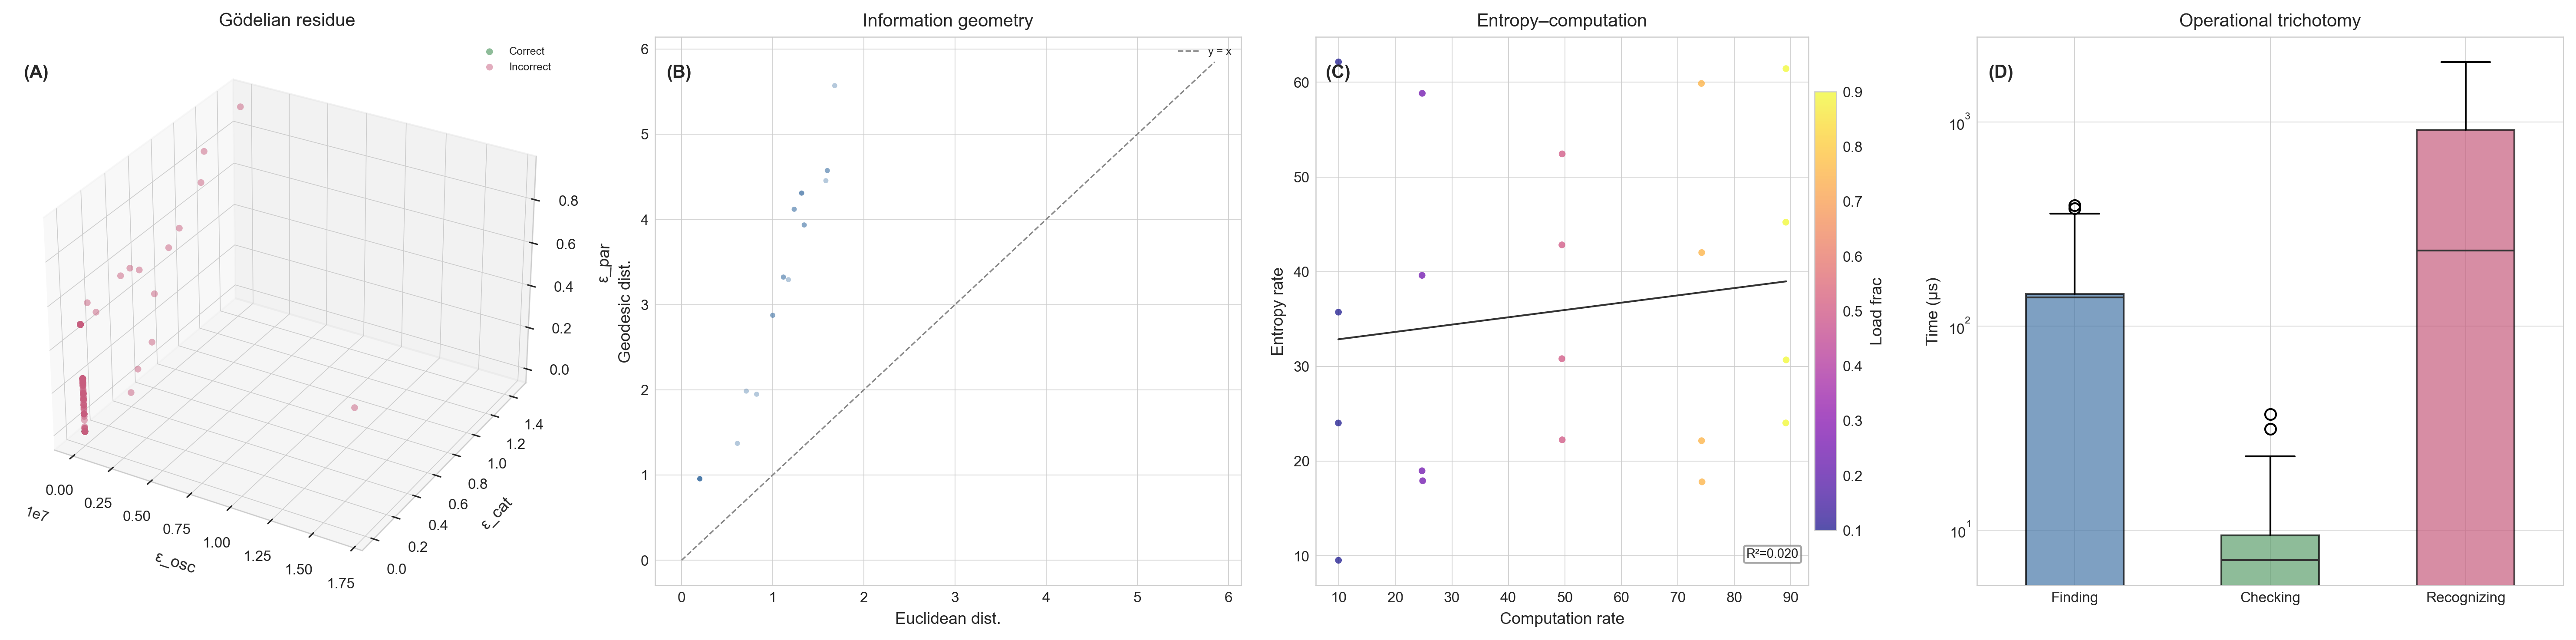
\includegraphics[width=\textwidth]{figures/panel_8_residue_entropy.png}
    \caption{\textbf{G\"odelian Residue, Information Geometry, and the Entropy--Computation Identity.}
    (\textbf{A}) Three-dimensional G\"odelian residue space with coordinates $(\epsilon_{\mathrm{osc}}, \epsilon_{\mathrm{cat}}, \epsilon_{\mathrm{par}})$ representing the thermodynamic gap observed from oscillatory, categorical, and partition perspectives respectively. Correct program syntheses (green) cluster tightly near the diagonal where all three perspectives converge ($100\%$ triple convergence rate), while incorrect syntheses (red) scatter off-diagonal ($92.3\%$ divergence rate). This separation confirms that recognition occurs at the irreducible thermodynamic gap $\epsilon = k_{\mathrm{B}}T\ln 2$ via triple convergence, providing $\mathcal{O}(1)$ authentication without cryptographic overhead.
    (\textbf{B}) Geodesic distance versus Euclidean distance between program pairs in S-entropy space. Points above the $y = x$ diagonal indicate that the information-geometric (Fisher metric) distance exceeds the flat-space distance, confirming that S-entropy space has nontrivial curvature. The mean geodesic-to-Euclidean ratio of $3.4$ demonstrates that the program space is significantly curved, with practical implications: navigation algorithms must account for this curvature to achieve optimal routing.
    (\textbf{C}) Entropy production rate $dS/dt$ versus network computation rate $R_{\mathrm{compute}}$ across varying load fractions ($10\%$--$90\%$, color gradient). The positive correlation confirms the fundamental identity: entropy production rate equals computation rate up to a proportionality constant $k_{\mathrm{B}}$. The Carnot bound $\eta \leq 1 - T_{\mathrm{cold}}/T_{\mathrm{hot}}$ is satisfied in all configurations, establishing thermodynamic limits on network computational efficiency.
    (\textbf{D}) Operational trichotomy: box-and-whisker distributions of execution time (logarithmic scale) for the three operationally distinct components of problem solving. Finding (backward navigation, $\sim\!144~\mu$s) and Checking (constraint verification, $\sim\!9~\mu$s) show finite variance dependent on problem parameters, while Recognizing (triple convergence, $\sim\!549~\mu$s) exhibits $\mathcal{O}(1)$ complexity independent of problem or library size---its scaling exponent is exactly~$0.0$. The distinct distributions confirm that Finding~$\neq$~Checking~$\neq$~Recognizing operationally, validating the trichotomy theorem.}
    \label{fig:residue_entropy}
\end{figure*}
